\chapter{Le deep learning en vision artificielle}
\label{chap:related-works}
Dans ce chapitre, nous décrivons les notions nécessaires de vision par ordinateur pour placer le contexte de notre travail. Nous faisons ensuite le lien entre l'utilisation du deep learning pour résoudre ces tâches et les nouvelles problématiques engendrées par cette utilisation.

% Classification d'image
\section{Classification d'images vs détection d'objets}
\label{sec:class-vs-detect}
Parmi les tâches de vision artificielle existantes, deux d'entre elles sont très populaires et ont de nombreuses applications. Ces deux techniques sont la classification d'images et la détection d'objets. Nous nous intéressons dans ce rapport à la détection, mais il est important pour la suite de comprendre également ce qu'est la classification.

\subsection*{Classification d'images}
Un algorithme de classification d'images \cite{classification-survey} prend une image en entrée dans le but de fournir une classe ou des probabilités d'appartenir à une classe en sortie. Les modèles de classification analysent les caractéristiques de l'entièreté de l'image afin de déterminer la classe. C'est pourquoi, habituellement, les images utilisées pour la classification présentent un seul objet à reconnaître en avant-plan avec un arrière-plan peu encombré. En générale, les performances d'un modèle de classification d'images sont mesurées via un taux de bonne reconnaissance sur les images de test d'un dataset.

\subsection*{Détection d'objets}
Un algorithme de détection \cite{Object-detection-survey} prend une image en entrée, détecte les instances des objets recherchés et fournit en sortie, pour chacun d'eux, une localisation au moyen d'une \textit{bounding box}\footnote{Boite englobante, en français.}. On peut citer comme exemple d'applications pratiques : la détection de défaut dans une texture \cite{7966162} ou encore la position d'objets dans une vitrine \cite{Sun2019ExploringBF}. Contrairement au problème de classification, la détection est un problème de régression. Il y a plusieurs difficultés en détection. Tout d'abord il faut analyser les caractéristiques de parties de l'image où peuvent se trouver une ou plusieurs instances d'objets recherchés. Et, ensuite, il faut fournir une bounding box placée de la manière la plus précise possible autour d'un objet détecté.


\begin{figure}[!h]
\centering
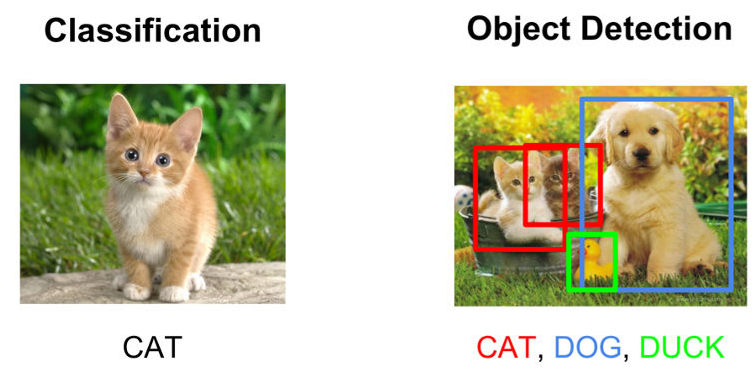
\includegraphics[scale=0.5]{img/Classi-vs-detect.PNG}
\caption{Exemple montrant la différence entre la détection et la classification. Source : \url{https://www.datacamp.com/community/tutorials/object-detection-guide}.}
\label{fig:class-vs-detec}
\end{figure}

\subsubsection*{Mesure de la performance d'un détecteur}
Les images d'apprentissage annotées, disponibles dans les datasets de détection, sont déjà munies de bounding boxes. Celles-ci sont connues sous le nom de "vérité terrain"\footnote{"ground truth", en anglais.}. Ainsi, pour quantifier la performance d'un détecteur, on utilise une mesure qui compare les bounding boxes trouvées à la vérité terrain. En général, les algorithmes de détection utilisent le \textit{mAP}\footnote{Mean Average Precision} \cite{hui_2018} pour mesurer la performance de la détection. En résumé, la mAP mesure la moyenne des surfaces des bounding boxes trouvées par le détecteur par rapport aux bounding boxes de la vérité terrain sur toutes les images et en tire un pourcentage.

\section{Détection d'objets et deep learning}
Avec le succès du deep learning en classification d'image \cite{im-class-nn}, les algorithmes de détection sur base du deep learning ont aussi eu une belle évolution. On peut classer les algorithmes de deep learning pour la détection d'objets en deux catégories :
\begin{itemize}
    \item \textbf{Détecteurs two-stage} \cite{R-CNN, Fast-RCNN, Faster-R-CNN} : ces algorithmes opèrent la détection en deux étapes (d'où le nom). Dans un premier temps, le détecteur identifie des régions d'intérêts (ROI\footnote{Region Of Interest}, en abrégé) qui sont susceptibles de contenir une instance d'un objet recherché. Ensuite, un classifieur discrimine ces ROIs pour déterminer si elles contiennent bel et bien un objet. Les détecteurs de type two-stage sont plus lents mais plus précis. Ils ne sont généralement pas adaptés pour du temps réel.
    \item \textbf{Détecteurs one-stage} \cite{YOLO, YOLO9000, YOLOv3, SSD, Retinanet} : ces algorithmes opèrent en une seule étape. Ils opèrent la détection sur un ensemble de localisations selon une grille pré-définie par l'utilisateur . Les détecteurs one-stage sont moins précis mais sont plus rapides. C'est pourquoi ils sont plus adaptés pour du temps réel.
\end{itemize}
Même si les détecteurs à base de deep learning sont actuellement les plus performants en terme de précision, ils ont également introduit un problème au niveau de la quantité d'images annotées manuellement à fournir. On peut voir, par exemple, des problèmes de détection \cite{COCO} avec plus de 330 000 images annotées pour détecter 80 classes d'objets. On peut donc constater que les algorithmes classiques de détection en deep learning requièrent une étape d'annotation manuelle très coûteuse qui peut s'avérer compliquée dans des conditions où on ne dispose pas d'assez de moyens.

% Transfer learning
\section{Transfer learning (TL)}
Une méthode pour pallier au manque d'image est le transfert learning. Le transfer learning consiste à entraîner un réseau de neurones en utilisant deux bases de données. Avec une première base de donnée, appelée la \textit{source}, on va pré-entraîner le réseau. Le but du pré-entraînement est de faire en sorte que le réseau apprenne à faire de l'extraction de caractéristiques sur des images (du type extraction des edges). On va ensuite apporter des modifications au réseau qui vont varier en fonction de l'objectif à atteindre. Enfin, on va entraîner le réseau modifié sur une base de données appelée la \textit{destination}. C'est dans la \textit{destination} que se trouvent les données qui vont nous permettre de résoudre le problème posé.

Dans le principe, la source sera un dataset très grand comme ImageNet \cite{ILSVRC15} avec plusieurs millions d'images qui permettra un entraînement du réseau avec une très grande efficacité. En effet, un réseau a besoin de beaucoup de données pour apprendre et, plus il a d'image, meilleur sera l'apprentissage. La destination sera, quant à elle, la base considérée qui sera généralement de petite taille. Pour des problèmes pratiques, une base de données de petite taille sera inférieure à 5000 images mais de nombreux travaux de recherche considèrent que des bases de données qui sont inférieures à 20000 images sont aussi de petite taille.

Les modifications doivent permettre de reprendre une partie de l'analyse faite par le réseau sur les données sources que la plupart des travaux supposent être les mêmes ou proches de celles sur les données de destination.

Il existe différentes approches de transfer learning qui prennent en compte l'objectif voulu, le type de réseau utilisé ou les données disponibles.

D'autres techniques prennent en compte le \textbf{type de réseau}. Certaines techniques sont spécifiques aux réseaux les plus grands (les \textit{profonds}) \cite{DBLP:journals/corr/abs-1804-06275} et certains sont même spécialisés pour les réseaux Deep que l'on appelle des "réseaux adverses" \cite{DBLP:journals/corr/CaoL0J17}.

Les techniques de transfer learning qui prennent en compte les \textbf{bases de données} sont des techniques qui vont s'appuyer sur le nombre d'images dans la destination \cite{Sun_2019_CVPR}, les différences entre la base source et destination et le fait que l'on puisse avoir plusieurs sources ou plusieurs destinations \cite{Dwivedi_2019_CVPR}. C'est ce genre d'approche qui a donné lieu au développement du \textbf{Few-Shot learning}, qui est une approche que nous détaillons dans le chapitre \ref{chap:FSOD}.

\hspace{1pt}
\par\noindent\rule{\textwidth}{0.4pt}

Les problèmes liés à l'utilisation du deep learning en vision artificielle décrits dans ce chapitre montrent le besoin de développer de nouvelles techniques, notamment pour réduire le nombre d'images à annoter à la main à fournir pour entraîner ces réseaux. Nous introduisons deux approches pour régler ce problème : le transfer learning et le few-shot learning. Dans la suite du rapport, nous décrivons ces deux approches et synthétisons les méthodes récentes dans ces domaines.